\documentclass[a4paper]{article}
\usepackage[margin=2cm]{geometry}
\usepackage{graphicx}
\usepackage{enumitem}
\setlist[description]{}

\begin{document}

\title{Torneos de Yu-Gi-Oh}
\author{
  \begin{tabular}{c}
    Chavely 02110766835 \\
    Jos\'e Carlos CI \\
    L\'azaro David CI \\
    Max CI
  \end{tabular}
}
\date{\today}
\maketitle
\newpage

\section{Diccionario de datos}

\newpage

\section{Esquema con el dise\~no de la aplicaci\'on}

\newpage

\section{Esquema de las clases definidas}

\begin{figure}[h]
  \centering
  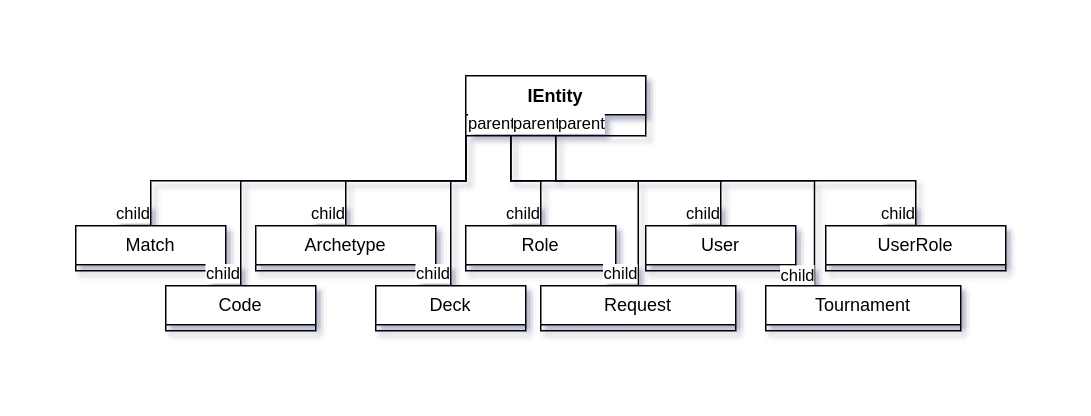
\includegraphics[width=1\textwidth]{ClasesDefinidas.png}
  \label{fig:etiqueta}
\end{figure}

\newpage

\section{Modelo conceptual de la base de datos:}

\newpage

\section{No s\'e k est\'an pidiendo en cada secci\'on peo m parece k tiene k ver con estas imgs so, aca se las dejo.}

\begin{figure}[h]
  \centering
  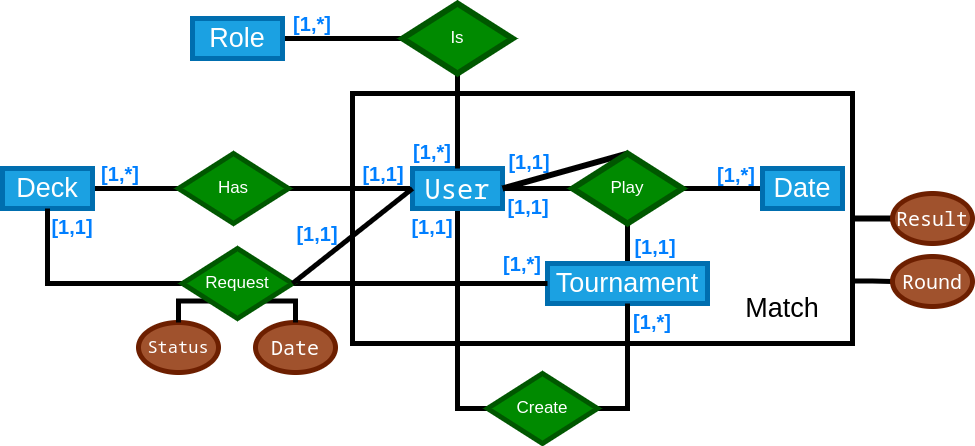
\includegraphics[width=1\textwidth]{merx.png}
  \caption{Esquema Relacional}
  \label{fig:etiqueta}
\end{figure}
\begin{figure}[h]
  \centering
  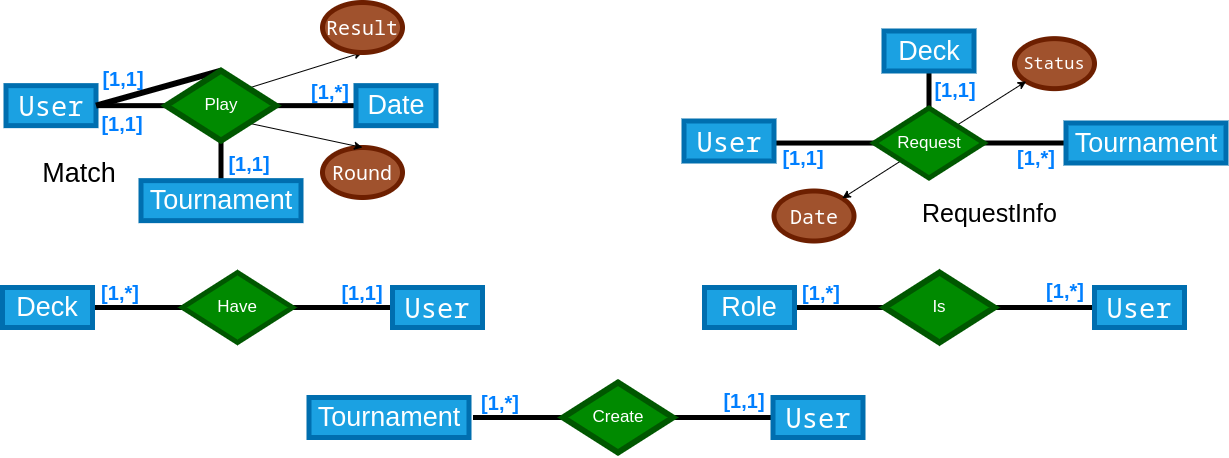
\includegraphics[width=1\textwidth]{relations.png}
  \caption{Esquema Relacional separado por relaciones}
  \label{fig:etiqueta}
\end{figure}

\begin{figure}[h]
  \centering
  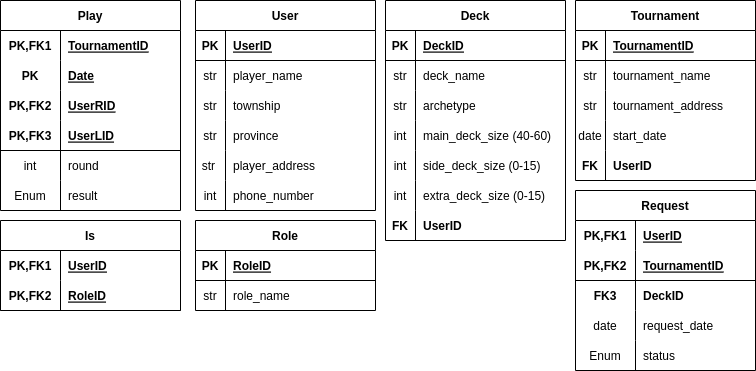
\includegraphics[width=1\textwidth]{table.png}
  \label{fig:etiqueta}
\end{figure}

\end{document} 
